\documentclass[10pt, a4paper]{ReportSheet}

%%%%% Preamble with packages
%%%%% ---------------------------------------------------------------
%%%%% Encoding and fonts
%%%%% ---------------------------------------------------------------
\usepackage[utf8]{inputenc}

% hyperlinks break on hyphens
\PassOptionsToPackage{hyphens}{url}

%%%%% Other packages
%%%%% ----------------------------------------------------------------
\usepackage{amsthm}
\usepackage{bm}
\usepackage{graphicx}
\usepackage[labelfont=bf]{caption}
\newcommand{\sourceDefaultLabel}{Author's elaboration}
\newcommand{\sourceLabel}{Source:}
\newcommand{\source}[1][\sourceDefaultLabel]{\caption*{\hfill\footnotesize{\sourceLabel~\textit{#1}}}}
\usepackage{psfrag}
\usepackage{fancyvrb}
\usepackage[numbers]{natbib}
\usepackage{usebib}
\usepackage{tikz}
\usepackage{bbding}
\usepackage{icomma}
\usepackage{dcolumn}
\usepackage{booktabs}
\usepackage{paralist}
\usepackage{float}
\newcommand\foreign[1]{\emph{#1}}
\usepackage{nameref}
\newcommand{\fullref}[1]{\textbf{\nameref{#1}}}

%%%%% Color boxes
%%%%% ---------------------------------------------------------------
\usepackage{tcolorbox}
% gray box preset
\newtcolorbox{gray-box}[1]{colback=gray!5!white,colframe=gray!50!black,title=#1}
% green box preset
\newtcolorbox{green-box}[1]{
    fonttitle=\bfseries,
    coltitle=black,
    colframe=blue!20!white,
    colback=blue!5!white,
    boxrule=0mm,
    title=#1
}
% answer box
\newcommand{\answerbox}[1]{
    \begin{green-box}{\MakeUppercase{\small{Odpověď}}}
        #1
    \end{green-box}
}

\setlength{\parindent}{0pt}

%%%%% Nastavení barev a syntaxe kódu
%%%%% ---------------------------------------------------------------
\usepackage{fvextra}
\usepackage{xcolor}
\definecolor{codekeyword}{rgb}{0.0,0.3,0.7}
\definecolor{codestring}{rgb}{0.4,0.4,0.8}
\definecolor{codecomment}{rgb}{0.2,0.2,0.2}
\definecolor{codejsdoc}{rgb}{0.4,0.4,0.4}
\definecolor{codelinenum}{rgb}{0.8,0.8,0.8}
\definecolor{lightyellow}{rgb}{255, 255, 224}

% nastavení minted balíčku
\usepackage[outputdir=dist]{minted}
\setminted{
    frame=none,
    breaklines=true,
    fontsize=\footnotesize,
    tabsize=2,
    linenos,
    numbersep=5pt,
    xleftmargin=0pt,
    baselinestretch=1.2,
    style=friendly,
%   TODO: highlihgting not working
    highlightcolor=\color{lightyellow},
    keywordstyle=\color{codekeyword},
    stringstyle=\color{codestring},
    commentstyle=\color{codecomment}\itshape,
    morecomment=[s][\color{codejsdoc}]{/**}{*/},
    numberstyle=\footnotesize\color{codelinenum}
}


%%%%% Hyperlink configuration
%%%%% ------------------------------------------------------------
\usepackage[unicode]{hyperref}
\usepackage{amsmath}
\hypersetup{pdftitle=MMAD - Úkol 1,
    pdfauthor=Filip Ditrich,
    ps2pdf,
    colorlinks=true,
    urlcolor=black,
    linkcolor=black,
    citecolor=black,
    pdfstartview=FitH,
    pdfpagemode=UseOutlines,
    pdfnewwindow,
    breaklinks
}
% make autoref links smaller and bold
\let\oldautoref\autoref
\renewcommand{\autoref}[1]{\small\textbf{\oldautoref{#1}}}

%%%%% Figures
%%%%% ---------------------------------------------------------------
\newcommand{\FIGDIR}{./assets/figures}

%%%%% Custom commands
% section with underline
\newcommand{\uloha}[5]{
    \section{Úloha #1\hfill\small\normalfont{(#2 body)}}
    \label{sec:uloha-#1}
    #3
    \subsection{Řešení}
    \label{subsec:uloha-#1-reseni}
    #4
    \ifthenelse{\equal{#5}{false}}{}{\newpage}
}

\usetikzlibrary{automata, positioning, arrows}

%%%%% Main document
%%%%% ------------------------------------------------------------
\begin{document}
%%% content
%%% --- title, author, date
    \title{MMAD - Úkol 1}
    \author{Filip Ditrich}
    \date{
        \footnotesize{
            \centering{
                Unicorn University, Prague, Czech Republic\\
                \today
            }
        }
    }
    \maketitle

% -- Úloha 1
    \uloha{1}{3}{
        Dokažte, že každá ortogonální matice má determinant $\pm 1$.
    }{
        Ortogonální matice je čtvercová reálná matice $Q$, která splňuje podmínku:
        \begin{equation*}
            Q^{TQ} = QQ^T = I
        \end{equation*}
        kde $I$ je jednotková matice.

        Dále platí, že determinant součinu dvou matic je roven součinu determinantů těchto matic, tedy:
        \begin{equation*}
            det(Q^{TQ}) = det(Q) \cdot det(Q^T)
        \end{equation*}

        Determinant jednotkové matice je vždy 1:
        \begin{equation*}
            det(I) = 1
        \end{equation*}

        Z předchozích vztahů plyne, že:
        \begin{equation*}
            det(Q^{TQ}) = det(I) = 1
        \end{equation*}

        Dá se také zapsat jako:
        \begin{equation*}
            det(Q) \cdot det(Q) = det(Q)^2 = 1
        \end{equation*}

        Odtud již plyne, že determinant ortogonální matice je roven $\pm 1$, jelikož:
        \begin{equation*}
            \sqrt{det(Q)^2} = \sqrt{1} = \pm 1
        \end{equation*}

        \answerbox{
            Ano, každá ortogonální matice má determinant $\pm 1$.
        }
    }

% -- Úloha 2
    \uloha{2}{3}{
        Pokud mají matice $A$ i $B$ stejná vlastní čísla, platí i, že $A \times B$ mají ty samá vlastní čísla?
    }{
        Neplatí. Uvažme matice
        \begin{equation*}
            A = \begin{pmatrix}
                    1 & 0 \\
                    0 & 2
            \end{pmatrix}
            \quad
            B = \begin{pmatrix}
                    2 & 0 \\
                    0 & 1
            \end{pmatrix}
        \end{equation*}
        Obě matice mají stejná vlastní čísla:
        \begin{equation*}
            \begin{aligned}
                det(A - \lambda I) &= 0 \Rightarrow (1 - \lambda)(2 - \lambda) = 0 \Rightarrow \lambda_1 = 1, \lambda_2 = 2 \\
                det(B - \lambda I) &= 0 \Rightarrow (2 - \lambda)(1 - \lambda) = 0 \Rightarrow \lambda_1 = 1, \lambda_2 = 2
            \end{aligned}
        \end{equation*}

        ale jejich součin:
        \begin{equation*}
            A \times B = \begin{pmatrix}
                             2 & 0 \\
                             0 & 2
            \end{pmatrix}
        \end{equation*}
        již vlastní čísla stejná nemají:
        \begin{equation*}
            det(A \times B - \lambda I) = det\begin{pmatrix}
                                                 2 - \lambda & 0           \\
                                                 0           & 2 - \lambda
            \end{pmatrix} = (2 - \lambda)^2 = 0 \Rightarrow \lambda = 2
        \end{equation*}

        Kdyby však matice $A$ a $B$ byly navzájem komutativní, tedy $A \times B = B \times A$, pak by platilo, že $A \times B$ mají stejná vlastní čísla jako $B \times A$, protože vlastní čísla matice jsou nezávislá na pořadí násobení:
        \begin{equation*}
            det(A \times B - \lambda I) = det(B \times A - \lambda I)
        \end{equation*}

        \answerbox{Ne, pokud matice $A$ a $B$ nemají stejná vlastní čísla, pak ani jejich součin $A \times B$ nemusí mít stejná vlastní čísla.}
    }

% -- Úloha 3
    \uloha{3}{3}{
        Rozhodněte, zda je následující matice diagonalizovatelná

        \[
            A = \begin{pmatrix}
                    0  & 1 & 2 \\
                    -4 & 1 & 4 \\
                    -5 & 1 & 7
            \end{pmatrix}
        \]
    }{
        Diagonalizovatelná matice je taková reálná čtvercová matice o rozměrech $n \times n$, která má $n$ navzájem různých
        vlastních čísel.

        Vlastní čísla matice $A$ jsou řešením rovnice $\det(A - \lambda I) = 0$:
        \begin{equation*}
            det(A - \lambda I) = \begin{vmatrix}
                                     -\lambda & 1           & 2           \\
                                     -4       & 1 - \lambda & 4           \\
                                     -5       & 1           & 7 - \lambda
            \end{vmatrix} = 0
        \end{equation*}

        Po úpravě dostaneme charakteristický polynom:
        \begin{equation*}
            p_A(\lambda) = -\lambda^3 + 8\lambda^2 - 17\lambda + 10 = 0
        \end{equation*}

        Tuto rovnici následovně upravíme:
        \begin{equation*}
            \begin{aligned}
                -\lambda^3 + 8\lambda^2 - 17\lambda + 10 &= 0 \\
                \cdots \\
                (\lambda - 1) \times (\lambda - 2) \times (\lambda - 5) &= 0
            \end{aligned}
        \end{equation*}

        A tím získáme kořeny charakteristické rovnice a tedy vlastní čísla matice $A$:
        \begin{equation*}
            \begin{aligned}
                \lambda_1 &= 1 \\
                \lambda_2 &= 2 \\
                \lambda_3 &= 5
            \end{aligned}
        \end{equation*}

        Jelikož $\lambda_1 \ne \lambda_2 \ne \lambda_3$, matice $A$ má 3 různá vlastní čísla a tedy je diagonalizovatelná.
        \answerbox{
            Ano, matice $A$ je diagonalizovatelná.
        }
    }

% -- Úloha 4
    \uloha{4}{3}{
        Nalezněte vlastní vektor příslušný k nejmenšímu a největšímu vlastnímu číslu matice $A$ z předchozího příkladu.
    }{
        Vlastní vektory matice $A$ jsou řešením soustavy rovnic $(A - \lambda I)x = 0$, kde $\lambda$ je vlastní číslo matice $A$.

        Nejmenší a největší vlastní čísla matice $A$ jsou $\lambda_{\min} = 1$ a $\lambda_{\max} = 5$.

        Pro $\lambda_{\min} = 1$:
        \begin{equation*}
            \begin{aligned}
            (A - 1I)
                x &= \begin{pmatrix}
                         -1 & 1 & 2 \\
                         -4 & 0 & 4 \\
                         -5 & 1 & 6
                \end{pmatrix} \begin{pmatrix}
                                  x_1 \\
                                  x_2 \\
                                  x_3
                \end{pmatrix} = \begin{pmatrix}
                                    0 \\
                                    0 \\
                                    0
                \end{pmatrix}
            \end{aligned}
        \end{equation*}

        Po úpravě dostaneme:
        \begin{equation*}
            \begin{aligned}
                x_1 - x_3 &= 0 \\
                x_2 + x_3 &= 0
            \end{aligned}
        \end{equation*}

        Řešením této soustavy rovnic je vlastní vektor $p$:
        \begin{equation*}
            p = \begin{pmatrix}
                    1  \\
                    -1 \\
                    1
            \end{pmatrix}
        \end{equation*}

        Pro $\lambda_{\max} = 5$:
        \begin{equation*}
            \begin{aligned}
            (A - 5I)
                x &= \begin{pmatrix}
                         -5 & 1  & 2 \\
                         -4 & -4 & 4 \\
                         -5 & 1  & 2
                \end{pmatrix} \begin{pmatrix}
                                  x_1 \\
                                  x_2 \\
                                  x_3
                \end{pmatrix} = \begin{pmatrix}
                                    0 \\
                                    0 \\
                                    0
                \end{pmatrix}
            \end{aligned}
        \end{equation*}

        Po úpravě dostaneme:
        \begin{equation*}
            \begin{aligned}
                x_1 - \frac{1}{2}x_3 &= 0 \\
                x_2 - \frac{1}{2}x_3 &= 0
            \end{aligned}
        \end{equation*}

        Řešením této soustavy rovnic je vlastní vektor $s$:
        \begin{equation*}
            s = \begin{pmatrix}
                    \frac{1}{2} \\
                    \frac{1}{2} \\
                    1
            \end{pmatrix}
        \end{equation*}

        \answerbox{
            Vlastní vektor příslušný nejmenšímu vlastnímu číslu $\lambda_{\min} = 1$ je $p = (1, -1, 1)^T$ a vlastní
            vektor příslušný největšímu vlastnímu číslu $\lambda_{\max} = 5$ je $s = \left(\frac{1}{2}, \frac{1}{2}, 1\right)^T$.
        }
    }

% -- Úloha 5
    \uloha{5}{3}{
        Mějme stálý migrační proces obyvatel mezi Severem, Jihem, Východem a Západem, jehož průběh za 1 rok lze znázornit diagramem níže (desetinná čísla udávají, jaký zlomek populace se za rok přemístí po šipce do jiné oblasti). Na počátku je počet obyvatel ve všech oblastech 10 milionů.

        Jak bude situace rozložení populace vypadat za 10 let od počátku? Na kterých hodnotách se populace v jednotlivých oblastech ustálí, pokud ji budeme dostatečně dlouho sledovat? Využijte libovolný počítačový nástroj a své argumenty podpořte výstupy tohoto nástroje.

        \begin{figure}[H]
            \centering
            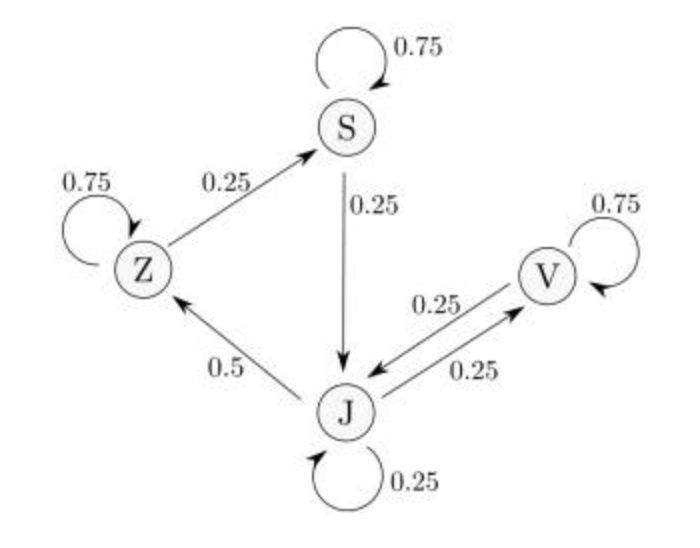
\includegraphics[width=0.5\textwidth]{\FIGDIR/ukol-1-5-diagram}
            \caption{Diagram stálého migračního procesu obyvatel mezi Severem, Jihem, Východem a Západem.}
            \label{fig:population-migration}
        \end{figure}
        \source{}
    }{
        ...
        \answerbox{–}
    }

% -- Úloha 6
    \uloha{6}{3}{
        Na adrese \url{https://openmv.net/file/room-temperature.csv} naleznete soubor s daty. Jedná se o simulovaná data měření teploty v místnosti. Data jsou v .csv formátu. Obsahují hlavičku a pět sloupců. V prvním sloupci je datum, v následujících čtyřech sloupcích jsou teploty měření v jednotlivých čtyřech rozích místnosti.

        Celkem je v souboru 144 záznamů měření. Pokud bychom chtěli s takovými daty dále pracovat, kolik hlavních komponent (a jaké) je vhodné zvolit a proč?
        Využijte SVD rozkladu a libovolného počítačového nástroje a své argumenty podpořte výstupy těchto nástrojů. Nezapomeňte na úvodní transformaci dat.
    }{
        Pro vyřešení této úlohy využijeme jazyk Python a knihovny \texttt{pandas} a \texttt{numpy} pro práci s
        maticemi a vektory.
    }{false}
% answer must be outside the \uloha command, since \minted cannot be used inside it
    Nejprve načteme data z CSV souboru a provedeme úvodní transformaci dat.
    \begin{minted}{python}
            import pandas as pd
            import numpy as np

            # načtení dat
            data = pd.read_csv('room-temperature.csv')
            # zahození sloupce s datem (nepotřebné pro analýzu)
            data = data.drop(columns=['date'])
            # normalizace dat (odstranění průměru)
            data = data - data.mean()
    \end{minted}

    Následně provedeme SVD rozklad matice dat a zjistíme, kolik hlavních komponent je vhodné zvolit.
    \begin{minted}{python}
            # SVD rozklad
            U, s, V = np.linalg.svd(data, full_matrices=False)
            # s = [34.54408633 16.15976563  7.69262365  6.51293724]

            # výpočet vysvětlené variance
            explained_variance = np.square(s) / np.sum(np.square(s))
            # explained_variance = [0.76688522 0.16782361 0.03803049 0.02726068]

            # zjištění počtu komponent pro 95% vysvětlené variance
            components = np.argmax(np.cumsum(explained_variance) > 0.95) + 1
            # components = 3
    \end{minted}


    \answerbox{
        Z výsledků SVD rozkladu zjistíme, že pro dosažení 95\% vysvětlené variance je vhodné zvolit 3 hlavní komponenty.
    }
    \newpage
\end{document}
